\documentclass[twoside]{article}
\usepackage{../estilo-ejercicios}
\newcommand{\x}{{\mathbf{x}}}
\newcommand{\y}{{\mathbf{y}}}
\usepackage[]{algorithm2e}
\usepackage{tikz-cd}
\usetikzlibrary{graphs}
\usetikzlibrary{arrows.meta,automata,positioning}
%--------------------------------------------------------
\begin{document}

\title{Optimización}
\author{Rafael González López}
\maketitle

\begin{ejercicio}{2.1}
Consideremos el grafo $G=(V,E)$ 
\[
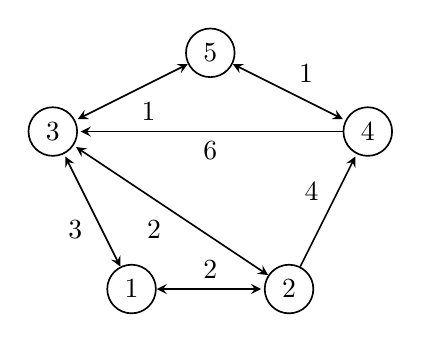
\begin{tikzpicture}[
    > = stealth, % arrow head style
    shorten > = 1pt, % don't touch arrow head to node
    auto,
    node distance = 3cm, % distance between nodes
    semithick % line style
    ]
\tikzset{every state}=[
    draw = black,
    thick,
    fill = white,
    minimum size = 1mm
    ]
    
    \node[shape=circle,draw=black] (A) at (1,0) {$1$};
    \node[shape=circle,draw=black] (B) at (3,0) {$2$};
    \node[shape=circle,draw=black] (C) at (0,2) {$3$};
    \node[shape=circle,draw=black] (D) at (4,2) {$4$};
    \node[shape=circle,draw=black] (E) at (2,3) {$5$};
         \path [<->] (E) edge  node {1} (C);
     \path [<->] (A) edge node {2} (B);
     \path [<->] (A) edge node {3} (C);
     \path [<->] (B) edge node {2} (C);
     \path [->] (D) edge node {6} (C);
     \path [<->](E) edge node {1} (D);
     \path [->](B) edge node {4} (D);
\end{tikzpicture}
\]
Aplicar el algoritmo de Dijkstra entre dos vértices.
\end{ejercicio}
\begin{solucion}
Vamos a calcular el camino más corto de $1$ a $4$
\begin{center}

\begin{tabular}{|c| c| c| c | c| c|}
\hline
Vértice & Paso 1 & Paso 2 & Paso 3 &  Paso 4 & Paso 5 \\
\hline
1 & $\infty$	& $\infty$ 	&  $(5,3)$  & $(6,2)$ &  \\
\hline
2 & $(4,4)$		& $\infty$ 	&  $(4,2)$ & $\boxed{(4,2)}$ &*\\
\hline 
3 & $\infty$ 	& $(2,5)$ 	& $\boxed{(2,5)}$ & * & *\\
 \hline
4 & $\boxed{(0,4)}$		& *& * & *&* \\
 \hline
5 & $(1,4)$		& $\boxed{(1,4)}$ & * &*&* \\
\hline
\end{tabular}\
\end{center}
Observamos que el camino que llevaba directamente desde $3$ a $1$ es de menor distancia que el que pasa por $2$. De esta forma, tenemos que el camino mínimo es $1-3-5-4$ con peso $5$.

\end{solucion}

\newpage



\begin{ejercicio}{2.2}
En el ejemplo visto en clase, ¿del 1 al 6 cuál es el coste y el camino?
\end{ejercicio}
Recordemos que la matriz de adyacencias del grafo está dada por
\begin{solucion}
$$
\begin{pmatrix}
0 		& 4 		& 7 		& 1 	& \infty 	& \infty\\
4 		& 0 		& \infty 	& 2 	& 6		 	& 3\\
7 		& \infty 	& 0 		& 3 	& \infty 	& 7\\
1 		& 2 		& 3 		& 0 	& 4 		& \infty\\
\infty 	& 6 		& \infty 	& 4 	& 0		 	& 1\\
\infty 	& 3 		& 7 		& \infty 	& 1 	& 0
\end{pmatrix}
$$
La matriz de distancias mínimas obtenidas por el algoritmo de Floyd es
$$
\begin{pmatrix}
0	& 3 	& 4 	& 1 	& 5		& 6\\
3  	& 0 	& 5 	& 2 	& 4		& 3\\
4  	& 5 	& 0 	& 3 	& 7 	& 7\\
1  	& 2 	& 3 	& 0 	& 4 	& 5\\
5 	& 4 	& 7 	& 4 	& 0		& 1\\
6 	& 3 	& 7 	& 5 	& 1 	& 0
\end{pmatrix}
$$
por tanto, el coste es 6 y es fácil ver que el camino es $1-4-5-6$.
\end{solucion}
\newpage
\begin{ejercicio}{2.3}
Consideremos el grafo $G=(V,E)$ dado por la matriz de distancias
$$
\begin{pmatrix}
0		& \infty 	& 3 		& \infty 	& \infty\\
4 		& 0			& \infty	& 1			& 2\\
3		& 8			& 0			& 2			& 6\\
\infty	& 1			& \infty	& 0			& 4\\
\infty	& 2,1		& 6			& 4			& 0
\end{pmatrix}
$$
\end{ejercicio}
Aplica el algoritmo de Floyd-Warshall.
\begin{solucion}
Consideramos la matriz de distancias y la matriz de recorridos
$$
\begin{pmatrix}
0		& \infty 	& 3 		& \infty 	& \infty\\
4 		& 0			& \infty	& 1			& 2\\
3		& 8			& 0			& 2			& 6\\
\infty	& 1			& \infty	& 0			& 4\\
\infty	& 1			& 6			& 4			& 0
\end{pmatrix}
\qquad
\begin{pmatrix}
-	& B 	& C 	& D 	& E\\
A	& -		& C		& D		& E\\
A	& B		& -		& D		& E\\
A	& B		& C		& -		& E\\
A	& B		& C		& D		& -
\end{pmatrix}
$$
Para no emborronar demasiado con los cálculos, mostraremos las matrices al final de las iteraciones. Para $k=1$ obtenemos
$$
\begin{pmatrix}
0		& \infty 	& 3 		& \infty 	& \infty\\
4 		& 0			& 7			& 1			& 2\\
3		& 8			& 0			& 2			& 6\\
\infty	& 1			& \infty	& 0			& 4\\
\infty	& 1			& 6			& 4			& 0
\end{pmatrix}
\qquad
\begin{pmatrix}
-	& B 	& C 	& D 	& E\\
A	& -		& A		& D		& E\\
A	& B		& -		& D		& E\\
A	& B		& C		& -		& E\\
A	& B		& C		& D		& -
\end{pmatrix}
$$
Para $k=2$
$$
\begin{pmatrix}
0		& \infty 	& 3 		& \infty 	& \infty\\
4 		& 0			& 7			& 1			& 2\\
3		& 8			& 0			& 2			& 6\\
5		& 1			& 8			& 0			& 3\\
5		& 1			& 6			& 2			& 0
\end{pmatrix}
\qquad
\begin{pmatrix}
-	& B 	& C 	& D 	& E\\
A	& -		& C		& A		& E\\
A	& B		& -		& D		& E\\
B	& B		& B		& -		& B\\
B	& B		& C		& B		& -
\end{pmatrix}
$$
Para $k=3$
$$
\begin{pmatrix}
0		& 11	 	& 3 		& 5 		& 9\\
4 		& 0			& 7			& 1			& 2\\
3		& 8			& 0			& 2			& 6\\
5		& 1			& 8			& 0			& 3\\
5		& 1			& 6			& 2			& 0
\end{pmatrix}
\qquad
\begin{pmatrix}
-	& C 	& C 	& C 	& C\\
A	& -		& C		& A		& E\\
A	& B		& -		& D		& E\\
B	& B		& B		& -		& B\\
B	& B		& C		& B		& -
\end{pmatrix}
$$
Para $k=4$
$$
\begin{pmatrix}
0		& 6		 	& 3 		& 5 		& 8\\
4 		& 0			& 7			& 1			& 2\\
3		& 3			& 0			& 2			& 5\\
5		& 1			& 8			& 0			& 3\\
5		& 1			& 6			& 2			& 0
\end{pmatrix}
\qquad
\begin{pmatrix}
-	& D 	& C 	& C 	& D\\
A	& -		& C		& A		& E\\
A	& D		& -		& D		& D\\
B	& B		& B		& -		& B\\
B	& B		& C		& B		& -
\end{pmatrix}
$$
Para $k=5$
$$
\begin{pmatrix}
0		& 6	 		& 3 		& 5 		& 8\\
4 		& 0			& 7			& 1			& 2\\
3		& 3			& 0			& 2			& 5\\
5		& 1			& 8			& 0			& 3\\
5		& 1			& 6			& 2			& 0
\end{pmatrix}
\qquad
\begin{pmatrix}
-	& D		& C 	& C 	& D\\
A	& -		& C		& A		& E\\
A	& D		& -		& D		& D\\
B	& B		& B		& -		& B\\
B	& B		& C		& B		& -
\end{pmatrix}
$$


\end{solucion}
\newpage

\begin{ejercicio}{2.4}
¿Cuál es el orden de complejidad del algoritmo de Floyd?
\end{ejercicio}
\begin{solucion}
Sea $G=(V,E)$ y sea $n=|V|$. En la etapa $i$ seleccionamos la $i$-ésima fila  y columna. Hacemos $n^2$ sumas y a lo sumo $n^2$ comparaciones y sutituciones. Este proceso se realiza para las $n$ filas, luego tenemos $2n^3$ operaciones. Por tanto, el algoritmo es $O(|V|^3)$.
\end{solucion}
\newpage

\begin{ejercicio}{2.5}
Comprobar que son equivalentes las caracterizaciones de árbol.
\begin{enumerate}
\item G es conexo y sin ciclos.
\item G es conexo y tiene $m-1$ aristas
\item G es conexo y al quitar un arco se vuelve disconexo.
\item G es no tiene ciclos pero al agregar una arista sí que lo tiene.
\item Para cada par de vértices solo existe un camino que los una.
\end{enumerate}
\end{ejercicio}
\begin{solucion}
\begin{proof}Veamos que cada punto implica el siguiente.
\begin{itemize}
\item Supogamos que $G$ es conexo y no tiene ciclos. Veamos que tiene $m-1$ aristas por inducción sobre $|V|=m$. Para $m=2$ es trivial. Supongamos que es cierto para $m-1$. Sea $G$ un grafo conexo sin ciclos y $m$ vértices. Dado que no tiene ciclos podemos considerar un camino de longitud máxima que claramente debe comenzar y acabar en hojas. Sea $v$ una de estas hojas. $G-v$ es un grafo conexo y sin ciclos (quitar una hoja no altera estas propiedades) con $m-1$ vértices. El resultado se sigue trivialmente.
\item Probémoslo por inducción. Para $m=2$ tenemos un único grafo conexo y al quitarle una arista se vuelve disconexo. Supongamos el caso base $m-1$. Sea $G$ un grafo conexo con $m$ vértices y $m-1$ aristas. Sea $e$ una arista de $G$. Si al quitar $e$ el grafo se vuelve disconexo, entonces hemos acabado. En caso contrario, tenemos que $G$ tiene un ciclo. Es fácil ver que si $G$ es conexo y tiene $m-1$ aristas no puede tener ciclos, pues necesitas como mínimo $m-1$ aristas para conectar $m$ vértices de manera que formen un grafo conexo.
\item Supongamos que $G$ es conexo y al quitar un arco se vuelve disconexo. No puede tener un ciclo, pues al quitar un arco, los vértices del ciclo siguen conectados. Si añadimos una arista $(u,v)$ y consideramos un camino de $u$ a $v$ que no use esa arista ($G$ ya era conexo), obtenemos un ciclo.
\item Consideremos 2 vérices cualesquiera $u,v$. Si son adyacentes entonces existe un camino y, dado que no existen ciclos, es único. Si no son adyacentes, consideremos el grafo añadiendo la arista $(u,v)$. Por hipótesis, ahora tenemos un ciclo $H$. Claramente $H-(u,v)$ es un camino en $G$ que conecta $u$ y $v$. Por el mismo razonamiento, es único.
\item Si existe un único camino que una cada par de vértices, en particular existe uno, por lo que $G$ es conexo. Además, si tuviese un ciclo, entonces para cualquier par de vértices de dicho ciclo existirían dos caminos. 
\end{itemize}
\end{proof}
\end{solucion}
\newpage

\begin{ejercicio}{2.6}
Ejemplo en el cual con un grafo de 4 o 5 nodos, unamos las parejas más baratas pero no las mejor.
\end{ejercicio}
\newpage

\begin{ejercicio}{2.7}
Aplicar el TSP al grafo de la última transparencia.
\end{ejercicio}
\newpage

\begin{ejercicio}{2.8} Aplicar el algoritmo Ford Fulkerson al grafo de las transparencias.
\end{ejercicio}
\begin{solucion}
Consideremos la matriz de las capacidades de flujo del grafo
$$
\begin{pmatrix}
0	&8	&4	&0	&0	&0\\
0	&0	&3	&3	&0	&0\\
0	&0	&0	&6	&2	&2\\
0	&0	&0	&0	&0	&6\\
0	&0	&0	&0	&0	&3\\
0	&0	&0	&0	&0	&0\\
\end{pmatrix}
$$
Aplicamos el algoritmo. Si escogemos del primer vértice la arista con flujo máximo y sucesivamente, obtenemos $1-2-3-4-6$. El peso mínimo que fluye es $k_1 = 3$. Por tanto consideremos la matriz actualizada
$$
\begin{pmatrix}
0	&5	&4	&0	&0	&0\\
0	&0	&0	&3	&0	&0\\
0	&0	&0	&3	&2	&2\\
0	&0	&0	&0	&0	&3\\
0	&0	&0	&0	&0	&3\\
0	&0	&0	&0	&0	&0\\
\end{pmatrix}
$$
Para la segunda iteración tendríamos el camino $1-2-4-6$, con flujo mínimo $k_2=3$.
$$
\begin{pmatrix}
0	&2	&4	&0	&0	&0\\
0	&0	&0	&0	&0	&0\\
0	&0	&0	&3	&2	&2\\
0	&0	&0	&0	&0	&0\\
0	&0	&0	&0	&0	&3\\
0	&0	&0	&0	&0	&0\\
\end{pmatrix}
$$
Ahora tendríamos $1-3-6$ con $k_3=2$, pues no hay manera de conectar $1$ con $6$ pasando por $2$ ni por $4$.
$$
\begin{pmatrix}
0	&2	&2	&0	&0	&0\\
0	&0	&0	&0	&0	&0\\
0	&0	&0	&3	&2	&0\\
0	&0	&0	&0	&0	&0\\
0	&0	&0	&0	&0	&3\\
0	&0	&0	&0	&0	&0\\
\end{pmatrix}
$$
Finalmente consideramos $1-3-5-6$ con $k_4=2$ y matriz
$$
\begin{pmatrix}
0	&2	&0	&0	&0	&0\\
0	&0	&0	&0	&0	&0\\
0	&0	&0	&3	&0	&0\\
0	&0	&0	&0	&0	&0\\
0	&0	&0	&0	&0	&1\\
0	&0	&0	&0	&0	&0\\
\end{pmatrix}
$$
Luego el flujo máximo es $k_1+k_2+k_3+k_4 = 10$.
\end{solucion}
\newpage
\end{document}